\documentclass[11pt,letter]{article}
\usepackage[top=1.00in, bottom=1.0in, left=1.1in, right=1.1in]{geometry}
\renewcommand{\baselinestretch}{1.1}
\usepackage{graphicx}
\usepackage{natbib}
\usepackage{amsmath}
\usepackage{hyperref}

\def\labelitemi{--}
\parindent=0pt

\begin{document}
\bibliographystyle{/Users/Lizzie/Documents/EndnoteRelated/Bibtex/styles/besjournals}
\renewcommand{\refname}{\CHead{}}

{\bf Updates on modeling species given their phylogenetic history in Stan}\\

\emph{Background \& Question:} A long line of evidence suggests phenological `sensitivity' in plants are likely driven in part by shared evolutionary history. As an example, pretend you're a tree who comes from a clade that for some reason in the past evolved to be responsive to variable spring temperatures. To be, effectively highly sensitive (you probably have high forcing, low chilling and low photoperiod cues to make this happen). You might move to a new climate where being less sensitive would be good, but because of your evolutionary history you're still pretty responsive. This would show up in models as a phylogenetic signal in your 'sensitivity' and if you drilled down, it should show up in your forcing. We want to know if there is evidence of this in plants as it would help us predict something about species for which we have no data and it would impose a constraint on how quickly we think these cues can evolve in the future. Lots of people have been interested in this before, but all work has used observational data. \\

So, given experimental data (hopefully removing confounding effects of geography on phenological dates) how much does phylogeny predict phenology? This question has some interesting embedded problems (or we could call them `opportunities') as we both the cues which inform the `sensitivity' and can use these to estimate phenological dates, and then assess the phylogenetic signal in dates, if we wanted---but now we're gotten perhaps very circular.\\

\emph{Common modeling approaches:} There are two really common approaches to questions like this: calculate Pagel's $\lambda$ on a trait, or correct for phylogenetic correlation in residuals in a typical analysis (PGLS) and analyse that correlation along the way (also called $\lambda$). These are {\bf not} necessarily identical: one is evaluating the correlation structure of a trait and one is calculating the correlation structure of residuals. Neither one of these is what we want because they are not the model we think is at play (see below) and because both reply on one trait value per species, but I think I should understand them to get anywhere. So let's do the PGLS, which I am copying from the second edition of \emph{Statistical Rethinking}.\\

\begin{align}
P & \sim MVN(\mu, S)\\
\mu_i & = \alpha +  \beta*F_i
\end{align}
$\mu$ is a usual linear model. $P$ is a vector of phenological dates (one per species), and $S$ is a covariance matrix with as many rows and columns as species. In ordinary regression this takes the form:
\begin{align}
S = \sigma^2I
\end{align}
where I is just an identity matrix (all 1s) so we can ignore it. In PGLS we replace $S$ with the phylogenetic covariance matrix. {\bf You have to make sure of a few things}: the phylogeny must go in as correlation matrix (this makes the diagonals 1s and the off-diagonals the correlation across species due to evolutionary history) and make sure the rows and columns are in the same order as the species will be ordered numerically. One issue with this model is that (I think) It force the correlation structure you give it---it does not adjust the correlation structure at all; some iterations of PGLS in certain R packages do this and it is quite an important addition to avoid Type I errors. I believe this just involves estimating a value to multiply the matix by such that:
\begin{align}
S = \sigma^2(I*\lambda)
\end{align}
So many models set $\lambda$ to 1, but it's definitely best to ask the model to estimate it (rather than assume the phylogenetic correlation strutcure if how you want to structure the residuals). \\

\emph{PMM (phylogenetic mixed model):} Here's my understanding:\\

\begin{align}
y & = \alpha + \beta x + a + e\\
a & \sim normal(0, \sigma_P^2\Sigma)\\
e & \sim normal(0, \sigma_R^2I)\\
\text{PGLS: }y & \sim normal(\mu + \beta x, \sigma_P^2\Sigma)
\end{align}
... where $\alpha$ and $\beta$, respectively, are the intercept and the slope for the co-factor x, $a$ is the phylogenetic random effect, and $e$ is the residual error. Now, the two last terms are assumed to be normally distributed, with $\Sigma$ as a phylogenetic correlation matrix , $I$ stands for the relevant identity matrix. Our model, thus, assumes that phylogenetic effects are correlated according to the phylogenetic correlation matrix $\Sigma$. Note also that our model is estimating two variances: $V_P$ is the variance of the phylogenetic effect and $V_R$ is the residual error (environment effects, intraspecific variance, measurement error, etc.). [This text here is copied from Chapter 11: General Quantitative Genetic Methods for Comparative Biology, by Villemereuil \& Nakagawa.]\\

The multiple-values-per-species version of this just involves within-group centering, which I don't see as necessary. \\

One interesting thing I noticed about this model is that it estimates a {\bf separate} intercept for the $y = \alpha + \beta x$ part of the model and I wonder if we need this?\\

\emph{My underlying model:} I think the phylogeny is a better option for partial pooling that treating species as under-ordered categories. I would ideally like a model that fits mainly the phylogeny, but also allows me to assess the strength of the phylogeny in the analysis. I sort of doubt we'll be able to manage this though. So I am searching for the best alternative option. \\

\emph{What we have tried:} So far, we have tried the following:
\begin{enumerate}
\item Fit the models with traditional partial pooling then estimate Pagel's $\lambda$ on species-level estimates of forcing, chilling, photoperiod. {\bf What's wrong with this?} We partially pool based on no structure among species (species with noisy and/or low sample size data will pool towards data-rich, low-noise species) so we could obliterate any signal. Plus it seems poor form to apply two different versions of species across analyses.
\item Try to fit PMM with brms. {\bf What's wrong with this?} I have no idea what brms is doing really.
\item Wrote my own Stan code that is not yet working (runs great, but does not estimate the phylogenetic effect correctly).  
\end{enumerate}

\begin{figure}[h!]
\centering
\noindent 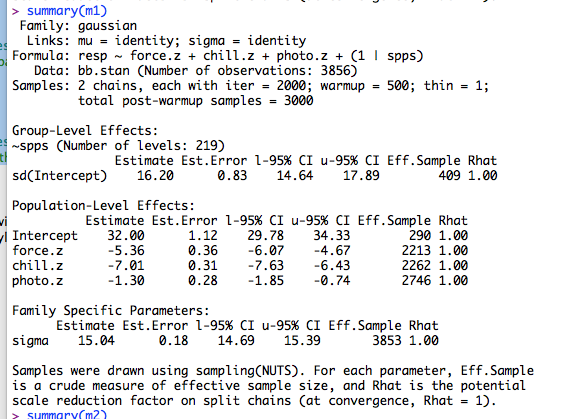
\includegraphics[width=0.8\textwidth]{figures/brms_m1.png} 
\caption{No phylogenetic structure, just species on the intercept.}
\end{figure}


\begin{figure}[h!]
\centering
\noindent 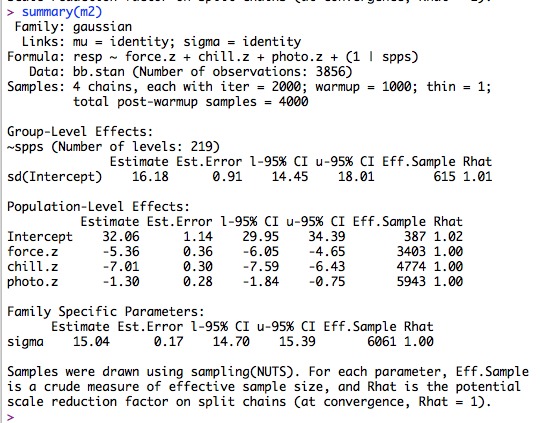
\includegraphics[width=0.8\textwidth]{figures/brms_m2.png} 
\caption{Adding phylogenetic structure (and species separately?) on the intercept.}
\end{figure}

\begin{figure}[h!]
\centering
\noindent 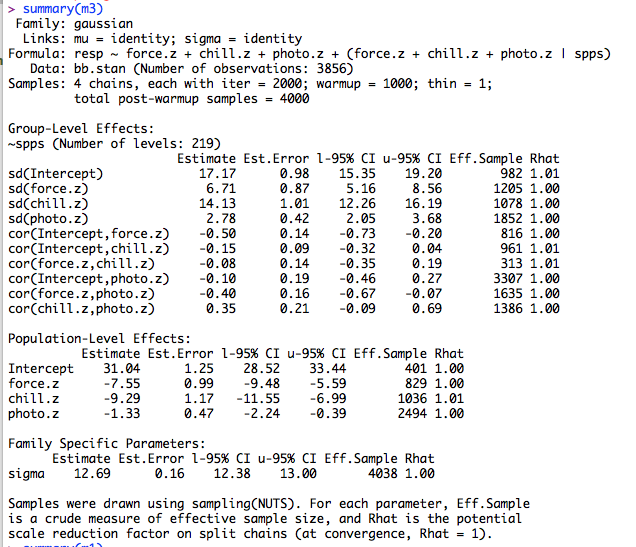
\includegraphics[width=0.8\textwidth]{figures/brms_m3.png} 
\caption{Adding phylogenetic structure and species on the intercept and slope? Or not ... not sure!}
\end{figure}

Some links:\\
\href{https://discourse.mc-stan.org/t/varying-slope-with-phylogenetic-structure/5739/4}{Varying slope with phylogenetic structure}\\
\href{https://discourse.mc-stan.org/t/multivariate-phylogenetic-with-repeated-measurements-model-help/14359/6}\\

\end{document}